%!TEX encoding = UTF-8 Unicode
% !TeX spellcheck = en_GB 
\special{papersize=8.5in,11in}
\documentclass[12pt]{article}
% \usepackage[active,tightpage]{preview}
%---- needed packages -------------------------------------------------
\usepackage{titling}
\usepackage{amsmath}
\usepackage{slashed}
\usepackage{amssymb}
\usepackage{epsfig}
\usepackage{graphicx}
\usepackage{multirow}
\usepackage{color}
\usepackage[normal]{subfigure}
\usepackage{rotating}
\usepackage{hyperref}
\usepackage[margin=1.0in]{geometry}
\usepackage[table]{xcolor}
\usepackage{enumitem}
\usepackage[utf8x]{inputenc}
\usepackage[compress,numbers,sort]{natbib}
\usepackage{authblk}
\usepackage{colortbl}
\usepackage{pdflscape}
\usepackage{color}
% \usepackage{hepunits}
\usepackage{hepnames}
\usepackage{numprint}
\usepackage{booktabs}
\usepackage{xparse}
\usepackage{mathrsfs}
\usepackage{bbold}
\usepackage{siunitx}
% Feynman diagrams
% \usepackage{/Users/lina/HEP/FeynArts/feynarts}
\usepackage{feynmp-auto}
\usepackage{tikz-feynman,tikz}

% \DeclareGraphicsRule{*}{mps}{*}{} % for being able to read the produced file
%\usepackage[utf8]{inputenc}
\unitlength = 1mm
\graphicspath{{./fig/}}
\definecolor{nicered}{rgb}{0.6,0.1,0.1}
\definecolor{nicegreen}{rgb}{0.1,0.5,0.1}
\definecolor{mediumcandyapplered}{rgb}{0.99, 0.12, 0.07}
\definecolor{red}{rgb}{1.0, 0, 0}
\hypersetup{colorlinks,citecolor= nicegreen,linkcolor= nicered}
\usetikzlibrary{shapes.callouts}
\usepackage{xparse}
\usetikzlibrary{decorations.text}
\definecolor{mygray}{RGB}{208,208,208}
\definecolor{mymagenta}{RGB}{226,0,116}
%~~~~~~~~~~~~~~~~~~~~~~~~~~~~~~~~~~~~~~~~~~~~~~~~~~~~~~~~~~~~~~~~~~~~~~~~~~~~~~
\tikzset{
	invisible/.style={opacity=0,text opacity=0},
	visible on/.style={alt=#1{}{invisible}},
	alt/.code args={<#1>#2#3}{%
		\alt<#1>{\pgfkeysalso{#2}}{\pgfkeysalso{#3}} % \pgfkeysalso doesn't change the path
		notice/.style  = { draw, rectangle callout, callout relative pointer={#1} },
	},
}
%~~~~

\usepackage[scale=2]{ccicons}
\usetikzlibrary{arrows,shapes}
\tikzstyle{every picture}+=[remember picture]
\newcommand*{\mytextstyle}{\sffamily\Large\bfseries\color{black!85}}
\newcommand{\arcarrow}[3]{%
	% inner radius, middle radius, outer radius, start angle,
	% end angle, tip protusion angle, options, text
	\pgfmathsetmacro{\rin}{1.7}
	\pgfmathsetmacro{\rmid}{2.2}
	\pgfmathsetmacro{\rout}{2.7}
	\pgfmathsetmacro{\astart}{#1}
	\pgfmathsetmacro{\aend}{#2}
	\pgfmathsetmacro{\atip}{5}
	\fill[mygray, very thick] (\astart+\atip:\rin)
	arc (\astart+\atip:\aend:\rin)
	-- (\aend-\atip:\rmid)
	-- (\aend:\rout)   arc (\aend:\astart+\atip:\rout)
	-- (\astart:\rmid) -- cycle;
	\path[
	decoration = {
		text along path,
		text = {|\mytextstyle|#3},
		text align = {align = center},
		raise = -1.0ex
	},
	decorate
	](\astart+\atip:\rmid) arc (\astart+\atip:\aend+\atip:\rmid);
}
%---- symbol short-hands and redefinitions -----------------------------
%%%%%%%%%%%%%%%%%%%%%%%%% referencing %%%%%%%%%%%%%%%%%%%%%%%%%%%%%%%%%
\def\eq#1{{Eq.~(\ref{#1})}}
\def\eqs#1#2{{Eqs.~(\ref{#1})--(\ref{#2})}}
\def\fig#1{{Fig.~\ref{#1}}}
\def\figs#1#2{{Figs.~\ref{#1}--\ref{#2}}}
\def\Table#1{{Table~\ref{#1}}}
\def\Tables#1#2{{Tables~\ref{#1}--\ref{#2}}}
\def\sect#1{{Sect.~\ref{#1}}}
\def\sects#1#2{{Sects.~\ref{#1}--\ref{#2}}}
\def\app#1{{Appendix~\ref{#1}}}
\def\apps#1#2{{Apps.~\ref{#1}--\ref{#2}}}
%%%%%%%%%%%%%%%%%%%%%%%%%%%%% math %%%%%%%%%%%%%%%%%%%%%%%%%%%%%%%%
\def\vev#1{\left\langle #1\right\rangle}
\def\abs#1{\left| #1\right|}
\def\mod#1{\abs{#1}}
\def\Im{\mbox{Im}\,}
\def\Re{\mbox{Re}\,}
\def\Tr{\mbox{Tr}\,}
\def\det{\mbox{det}\,}
\def\etal{\hbox{\it et al.}}
\def\ie{\hbox{\it i.e.}{}}
\def\eg{\hbox{\it e.g.}{}}
\def\etc{\hbox{\it etc}{}}
%%%%%%%%%%%%%%%%%%%%%%%%%%%%%
\newcommand{\neff}{n_{\rm eff}}
\renewcommand{\d}{{\rm d}}
\renewcommand{\bar}{\overline}
\newcommand{\hoppet}{\textsc{Hoppet}}
\newcommand{\R}[2]{$R_{#1#2}$}
%\newcommand{\as}{$\alpha_s$}
\newcommand{\rr}[1]{{\color{red}#1}}
\newcommand{\bb}[1]{{\color{blue}#1}}
\newcommand{\vs}{v_{\scriptscriptstyle S}}
\newcommand{\vh}{v_{\scriptscriptstyle H}}
\newcommand{\lambdah}{\lambda_{\scriptscriptstyle H}}
\newcommand{\muh}{\mu_{\scriptscriptstyle H}}

%%%%%%%%%%%%%%%%%%%%%%%%%%%% 2hdm shortcuts
\newcommand{\sinb}{\sin\beta}
\newcommand{\cosb}{\cos\beta}
\newcommand{\tb}{\tan\beta}
\newcommand{\ctb}{\cot\beta}
%\newcommand{\sba}{\sin\left(\beta-\alpha\right)}
%\newcommand{\cba}{\cos\left(\beta-\alpha\right)}
\newcommand{\sba}{s_{\beta-\alpha}}
\newcommand{\cba}{c_{\beta-\alpha}}
\newcommand{\SM}{\text{SM}}
%%%%%%%%%%%%%%%%%%%%%%%%%%%% commemnts by name, makes tracking easier
\definecolor{myv}{HTML}{885B8D}
\definecolor{darkpastelgreen}{rgb}{0.01, 0.75, 0.24}
\newcommand{\Ramona}[1]{\textcolor{red}{#1}}
\newcommand{\Lina}[1]{\textcolor{myv}{#1}}
%%%%%%%%%%%%%%%%%%%%%%%%%%%%%
\definecolor{LightCyan}{rgb}{0.88,1,1}
\definecolor{piggypink}{rgb}{0.99, 0.87, 0.9}
\definecolor{applegreen}{rgb}{0.55, 0.71, 0.0}
\definecolor{green-yellow}{rgb}{0.68, 1.0, 0.18}
\newcommand{\GeV}{\si{\GeV}}
\newcommand{\TeV}{\si{\TeV}}
\newcommand{\invab}{\si{\per \atto\barn}}
\newcommand{\femtobarn}{\si{\femto\barn}}
% \newcommand{\beq}{\begin{equation}}
% \newcommand{\eeq}{\end{equation}}
% \newcommand{\bea}{\begin{eqnarray}}
% \newcommand{\eea}{\end{eqnarray}}

\newcommand{\Red}[1]{{\color{nicered}{#1}}}
\newcommand{\published}[1]{%
\gdef\puB{#1}}
\newcommand{\puB}{}
\renewcommand{\maketitlehooka}{%
\par\noindent \puB}

%%%%%%%%%%%%% functions for eff  %%%%%%%%%%%

% % number of expected events theoretical 289
% \ExplSyntaxOn%
% % number of expected events theoretical 289
% \newcommand\eff[2]
%     { \fp_to_decimal:n { (#1)/(#2)) } }
% \ExplSyntaxOff
% \ExplSyntaxOn%
% \newcommand\poiserr[2]
%     { \fp_to_decimal:n { (#1)/(#2)* (1.0/(#1)+1.0/(#2))^0.5} }
% \ExplSyntaxOff


\title{\bf{Phenomenology of the Higgs and flavour in the Standard Model and beyond }}

\author{Lina Alasfar}
\author[2]
{Lina Alasfar \\  Supervisor: Prof. Dr Ramona Gr\"{o}ber}

%\affil[1]{\emph{\normalsize Humboldt-Universit\"at zu Berlin, Institut f\"ur Physik,
%Newtonstr.~15, 12489 Berlin,  Germany.}}
% \affil[2]{\emph{\normalsize CAFPE and Departamento de F\`isica T\'eorica y del Cosmos, Universidad de Granada, E18071 Granada, Spain.}}


\date{Doctoral Research Plan}
%\published{\flushright \vskip-0.5cm HU-EP-XX/YY}

%\published{\flushright \vskip1cm}

\begin{document}
\maketitle

\section*{Introduction}
Since the discovery of the Higgs particle in 2012 by a collaborative efforts between ATLAS~\cite{Aad:2012tfa} and CMS~\cite{Chatrchyan:2012xdj} experiments at the {\bf L}arge {\bf H}adron {\bf C}ollider~(LHC), and the Standard Model of particle physics has been completed,yet leaving many questions unanswered. After the discovery of the new particle,  a lot is to be known about  its precise mass, spin, $\mathcal{CP}$- parity and couplings. 
\begin{center}
	\begin{tikzpicture}
	\fill[even odd rule,myv] circle (1.5);
	\node at (0,0) [
	font  = \mytextstyle,
	color = white,
	align = center
	]{
		\textcolor{white}{ Higgs}
	};
	\arcarrow{ 85}{  3}{ Mass   }
	\arcarrow{270}{357}{ Width    }
	\arcarrow{182}{269}{ CP }
	\arcarrow{176}{ 96}{  Spin }
	\end{tikzpicture}
\end{center}
\par The mass of the Higgs has been measured to high precision~\textcolor{myv}{$ m_h=124.97 \pm 0.24$ GeV\xspace}~\cite{Aaboud:2018wps} . Moreover, the  $\mathcal{CP}$ properties ans spin are confirmed to be a scalar with even~$\mathcal{CP}$, though there is a small room left for the Higgs to be a mixture of $\mathcal{CP}$, even and odd states~\cite{Aad:2015mxa}. Higgs couplings to the SM gauge bosons has been measured with great accuracy~\cite{CMS-PAS-HIG-19-005} along with its coupling to the third generation quarks and leptons~\cite{Sirunyan:2017khh,Sirunyan:2019nlw,CMS-PAS-HIG-19-005},  they were found to agree with the SM prediction up to 10\% -- 20\% \cite{Aad:2019mbh}.  Making the upcoming years for the LHC,  years for precision measurements for the Higgs demanding more accurate calculations for Higgs-involved processes at higher perturbation theory orders in order to close in further the Higgs properties and couplings. As one of the major challenges in Higgs physics at higher luminosity runs of the LHC is the theoretical uncertainties of the calculated processes to be searched by experimentalists. \\
%%%%
\par Nevertheless, the couplings between the Higgs and first and second generations fermions , and its self couplings are not at the precision level. For instance, the trilinear coupling $ hhh$ scaling $\kappa_\lambda := \lambda_{hhh}/\lambda_{hhh}^{\SM}$ , has been constrained to be within the  $-5.0<\kappa_\lambda< 12.0 $, @ 95\% CL~\cite{Aad:2019uzh} .These limits and are still weaker than the~(theoretical) limits coming from perturbative unitarity~\cite{DiLuzio:2017tfn} and vacuum stability~\cite{Falkowski:2019tft}. While  the experimental bounds on $\kappa_\lambda$ could be improved in the search for double Higgs production at the High-Luminosity phase of the LHC~(HL-LHC),  the quartic coupling $hhhh$ will remain beyond the reach of the HL-LHC, similarly the complete determination of the Higgs width, as the current bound is $\Gamma/\Gamma^{SM }< 3.5$~\cite{CMS-PAS-HIG-18-002,Aaboud:2019rtt}.  The same situation is shared with the Higgs coupling to light fermions, particularly quarks. Since the SM prediction for Higgs couplings to be proportional to the mass of the particle, the couplings between the Higgs and fermion generations~(via Yukawa interaction) shows an unexplained hierarchy, see figure~\ref{yuk}.
 %
\begin{figure}[!htbp]
	\centering
	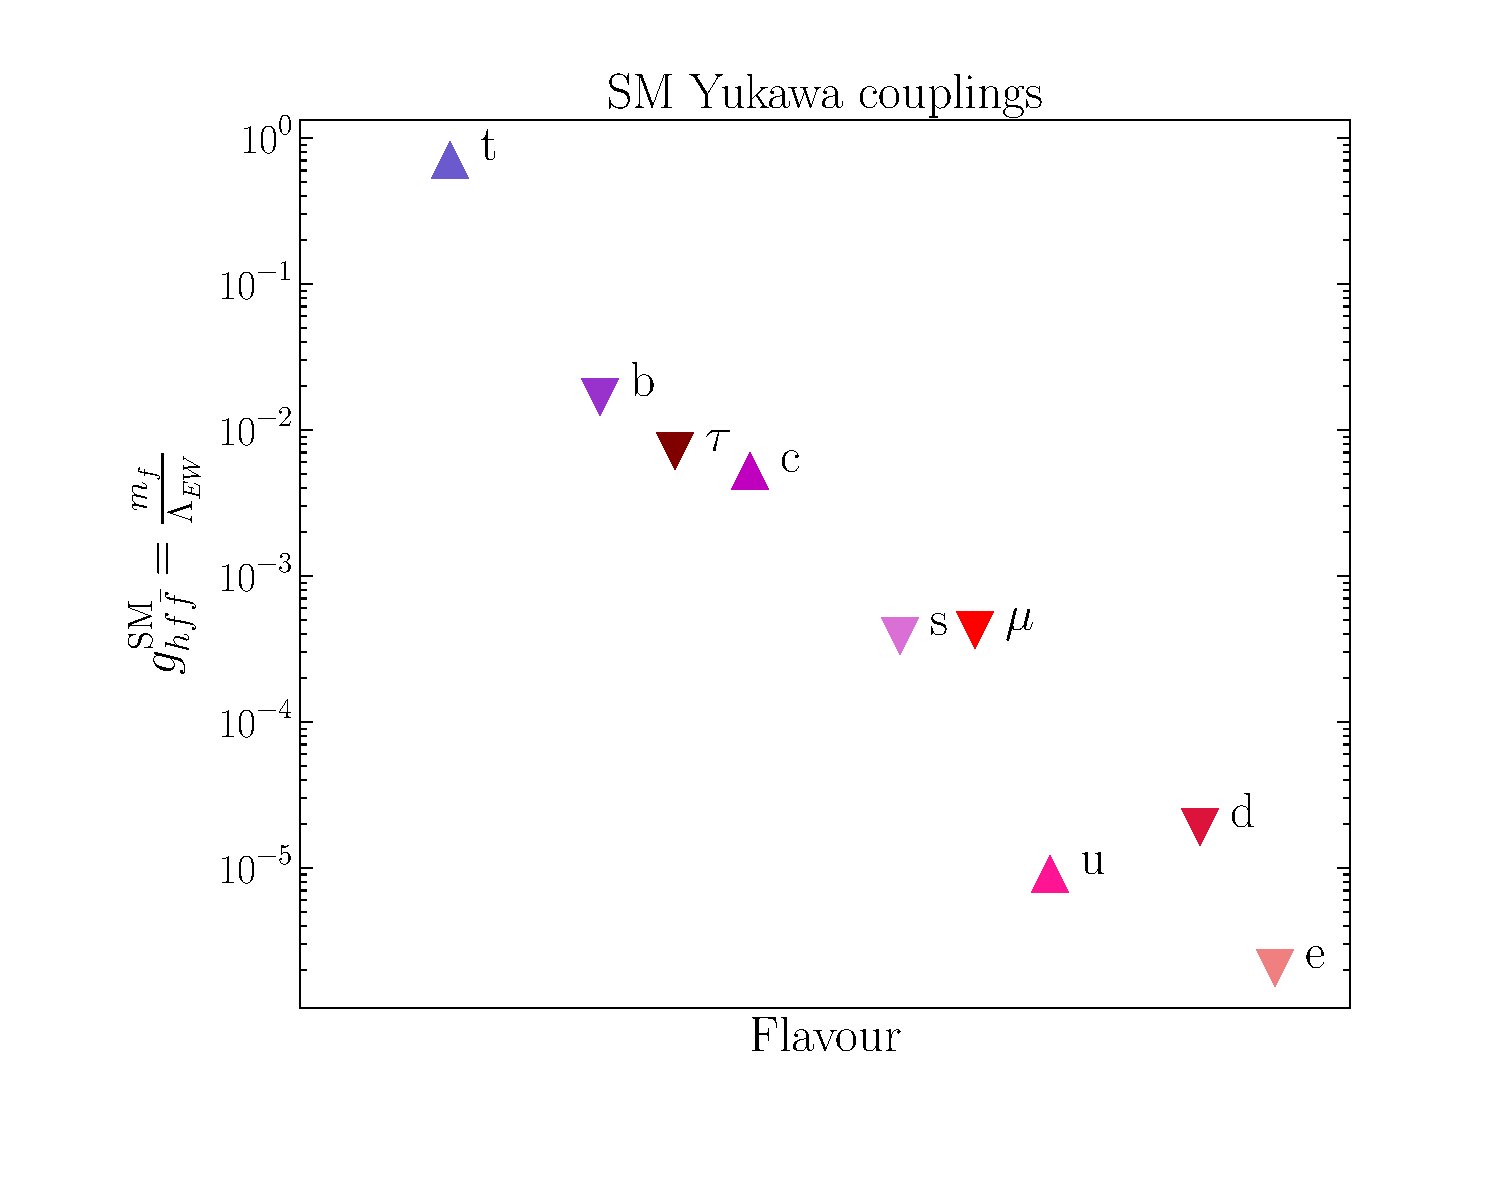
\includegraphics[scale=0.35]{yukawa}
	\label{yuk}
	\caption{The hierarchy between the Yukawa couplings amongst the fermion generations}
\end{figure}
%
This is known as the ``old" flavour puzzle~\footnote{Opposed to the ``New" flavour puzzle coming from the tension between SM prediction and recent LHCb measurements of lepton flavour universality in neutral semi-leptonic beauty meson decays. } of which the SM has no explanation for this unnatural Yukawa couplings. Moreover,due to the smallness of first and second generations masses, it presents the phenomenologists and experimentalists an extra challenge to constrain the light fermion couplings, even at the HL-LHC.  Current fits for  light quark Yukawa couplings depend on the ansatz of Higgs width, since the latter is beyond the reach of the LHC, they need to be made under assumptions~ \cite{Englert:2014aca,Caola:2013yja,Aaboud:2018puo, Sirunyan:2019twz}. Hence the current global fits are all model-dependent~\cite{deBlas:2019rxi} . 
 This flavour puzzle could be solved, even partially, by assuming a larger-yet unconstrained- Yukawa couplings between the Higgs and light fermions, by introducing new particles and symmetries. With carefully-selected processes investigated for the light fermion couplings with the Higgs, one could hope to investigate such models and make a model-independent fit for the these couplings at the HL-LHC that are comparable to (or even stronger) than the model-dependent fits. 
 %
 \par The double Higgs production will be the main process to look for at the HL-LHC, as it is expected to be sensitive to the SM $hh$ production at $2-3 \sigma$. The introduction of new couplings between top quark and the Higgs~(like with top partner) would enhance the $hh$ significantly~\cite{Dib:2005re, Grober:2010yv, Contino:2012xk, Grober:2016wmf}, possibly to $\sim 5 \sigma$. In addition to probing the trilinear coupling, the double Higgs production is an important process for probing no-linearity in the couplings between the Higgs and other SM particles, e.g. $hVV$ and $hhVV$ which is a feature of non-linear $\sigma$model which Composite Higgs model~(CHM) are based on. Moreover, the relation between the couplings $h \bar f f$ (Yukawa) and  $h h \bar f f$ also being non-linear in CHM with vector-like quark partners as illustrated in figure\ref{chm10}.
 \begin{figure}[!htbp]
 	\centering
 	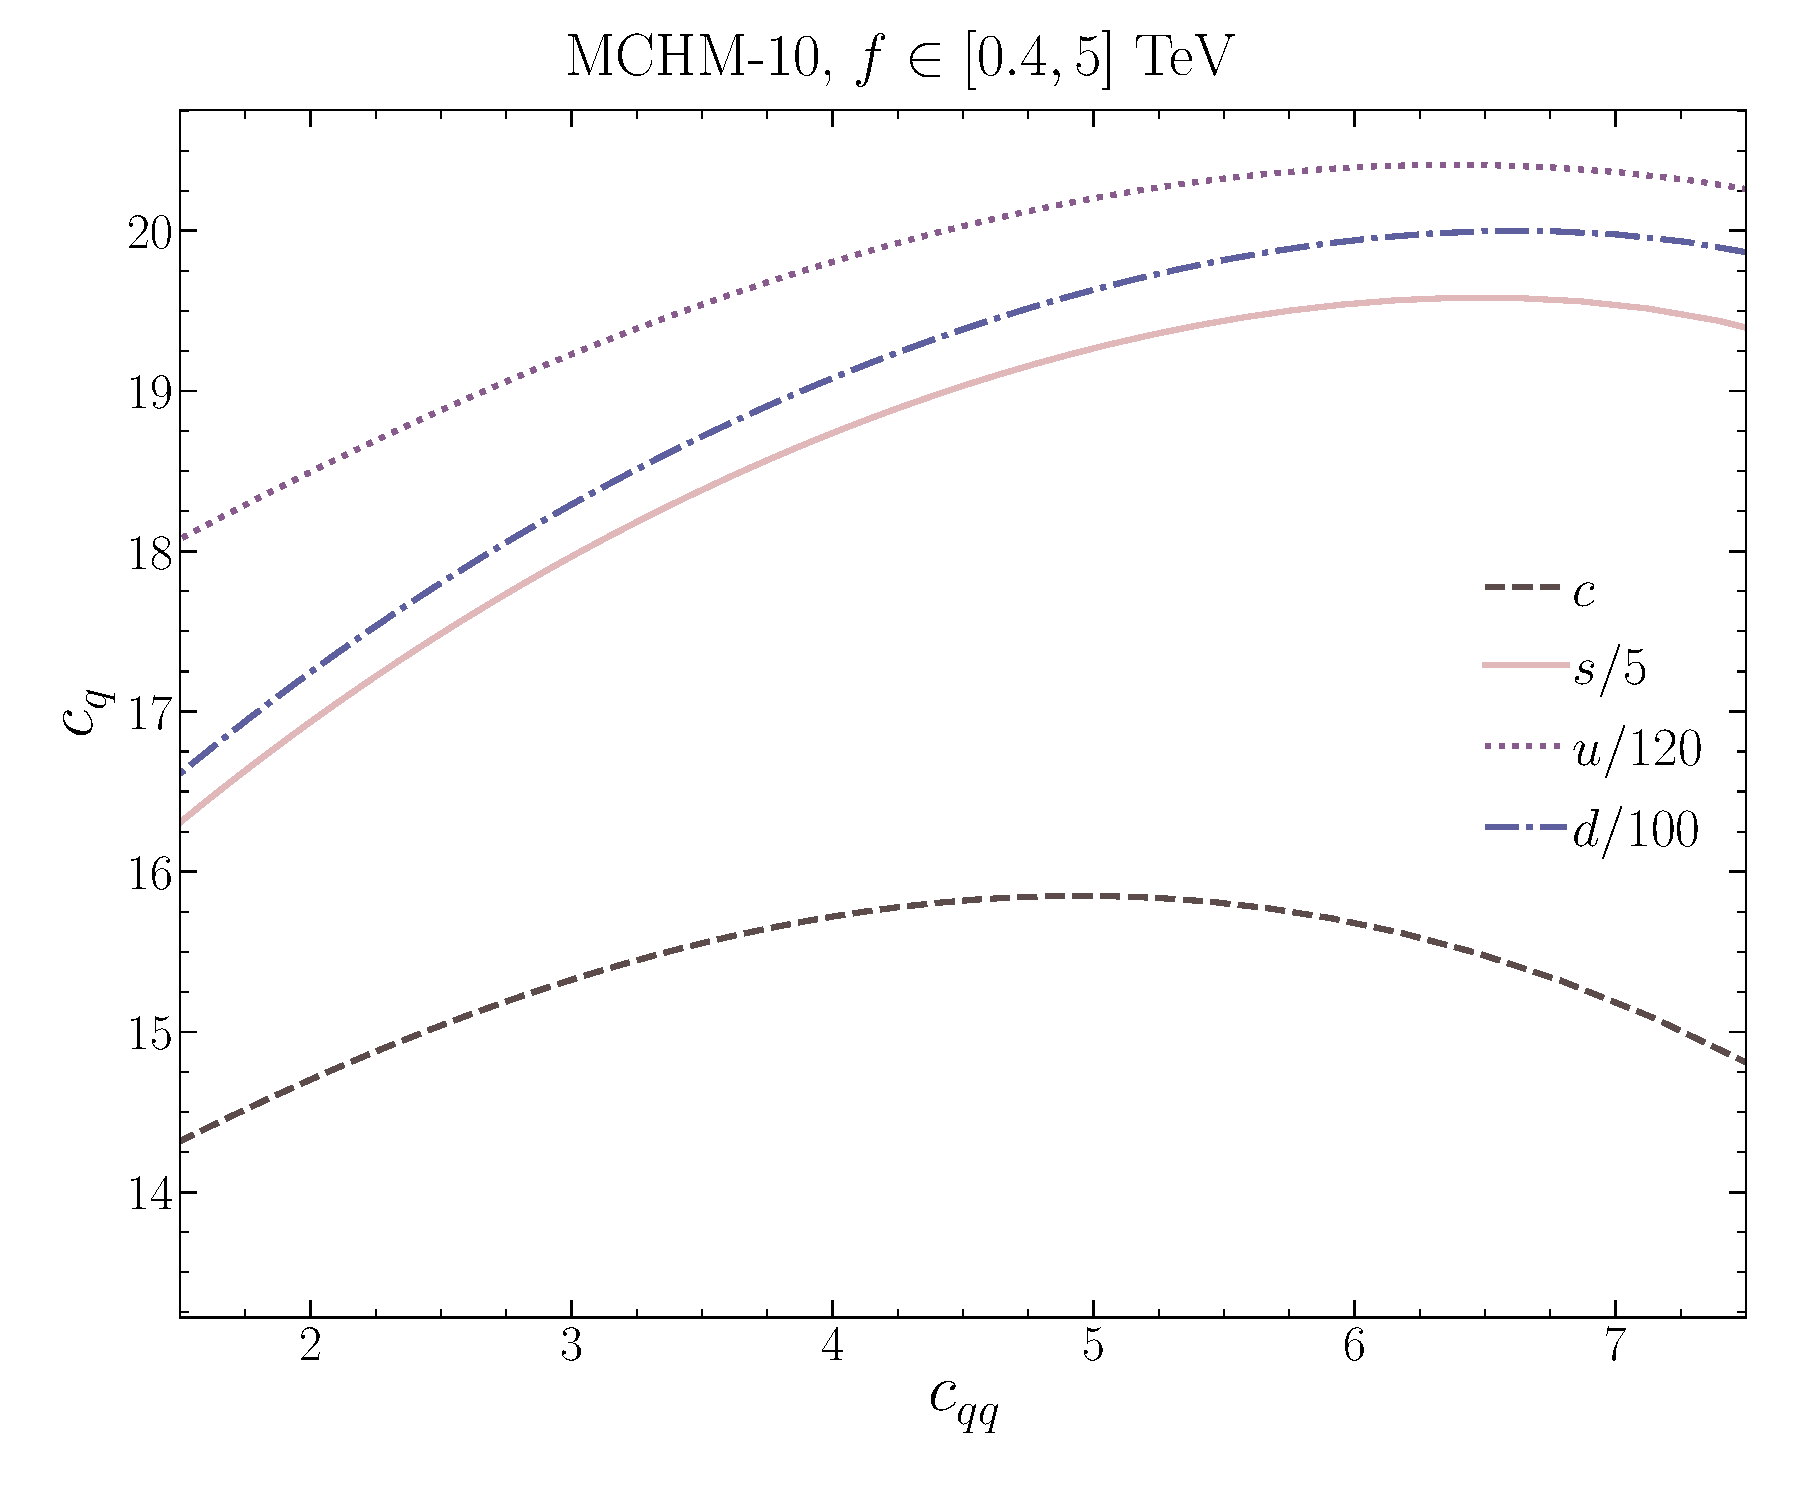
\includegraphics[scale=0.25]{chm_cqcqq}
 	\label{chm10}
 	\caption{The non-linearity between the matched Wilson coefficients~$ c_q$ and $ c_{qq}$, for the effective couplings ~$h \bar f f$ and $h \bar f f$,respectively; illustrated in a minimal composite Higgs model known as MCHM10, with light quark partners. }
 \end{figure}
\par It was proposed that one could look at other ways to probe the trilinear coupling, coming from electroweak corrections and constrain Standard Model effective field theory (SMEFT) operators modifying $\lambda_{hhh}$, form currently observed processes~\cite{Hartland:2019bjb}. However, fitting with SMEFT should be done carefully, as the introduction of different operators could dilute the original operators of concern. Hence, this should be studied further. 
 
 \section*{The doctoral thesis}
 The doctoral thesis will be composed of multiple, almost independent, research projects. The main focus of these projects is Higgs and flavour phenomenology at the LHC and HL-LHC. The currently suggested projects are\\ \bigskip\\
 \begin{minipage}{0.75\linewidth}
 \begin{itemize}
 	\item Probing Higgs couplings to light quarks via Higgs pair production
 	\item Next-to-leading order~(NLO) QCD correction to $Zh$ production via gluon fusion  with full top mass effect. \\ This project also involves an investigation of the potential contribution of ggF Drell-Yan-like process$ gg \to Z^* \to \bar L L$ where $L$ is a new heavy leptonic state. The  2 loop correction to be made for the triangle diagram.
 	\item One-loop New Physics scenarios for $b \to s$ anomalies: Combining EW and Flavour constraints in the SMEFT \\ Involving model building inspired by composed Higgs models. 
 	\item Model building for modifying the light quark/lepton couplings with the Higgs 
 	\item Investigation of the process $  pp \to h W^+ W^-$  with modified  light Yukawa coupling .
 	\item SMEFT study for EW corrections to the single Higgs production as a potential probe for trilinear coupling.
 \end{itemize}
 \end{minipage}
 \begin{minipage}{ 0.25\linewidth}
	\begin{center}
		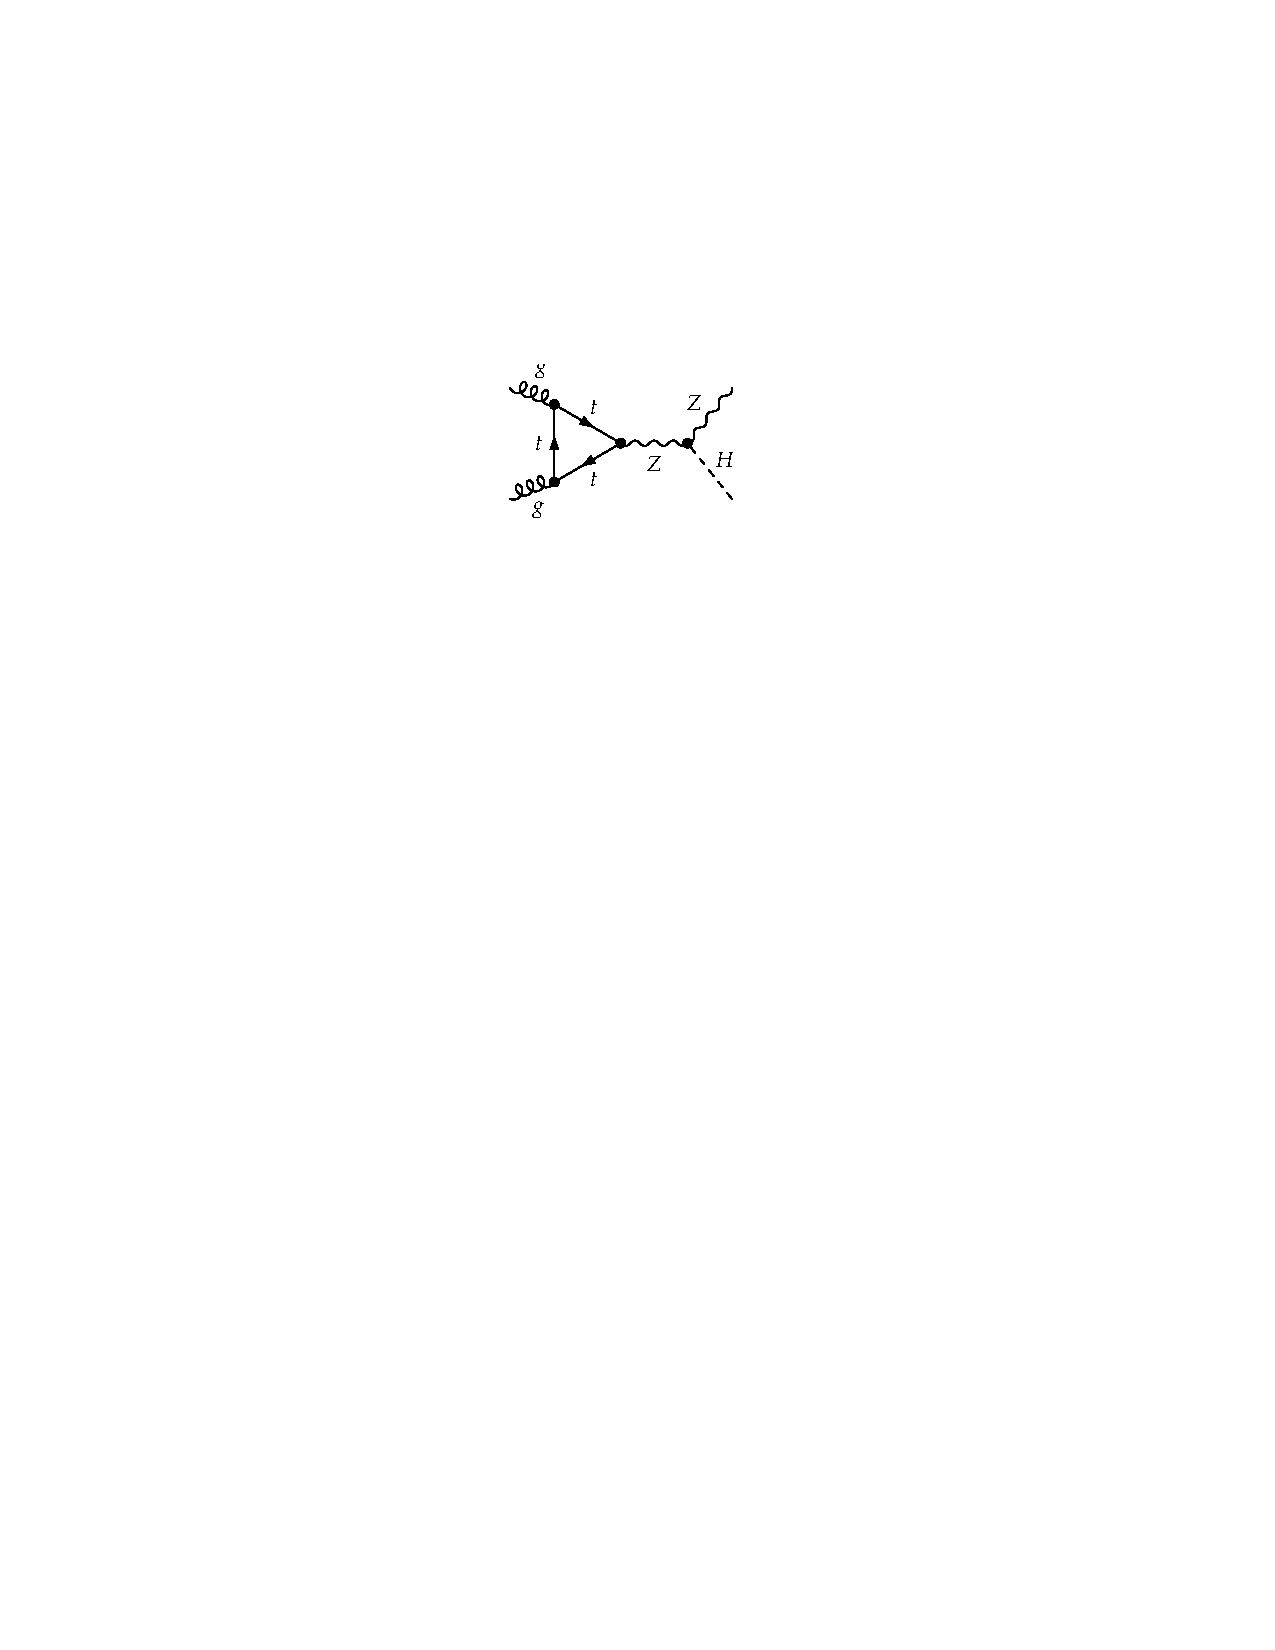
\includegraphics[width=1\textwidth]{1loop} \\
		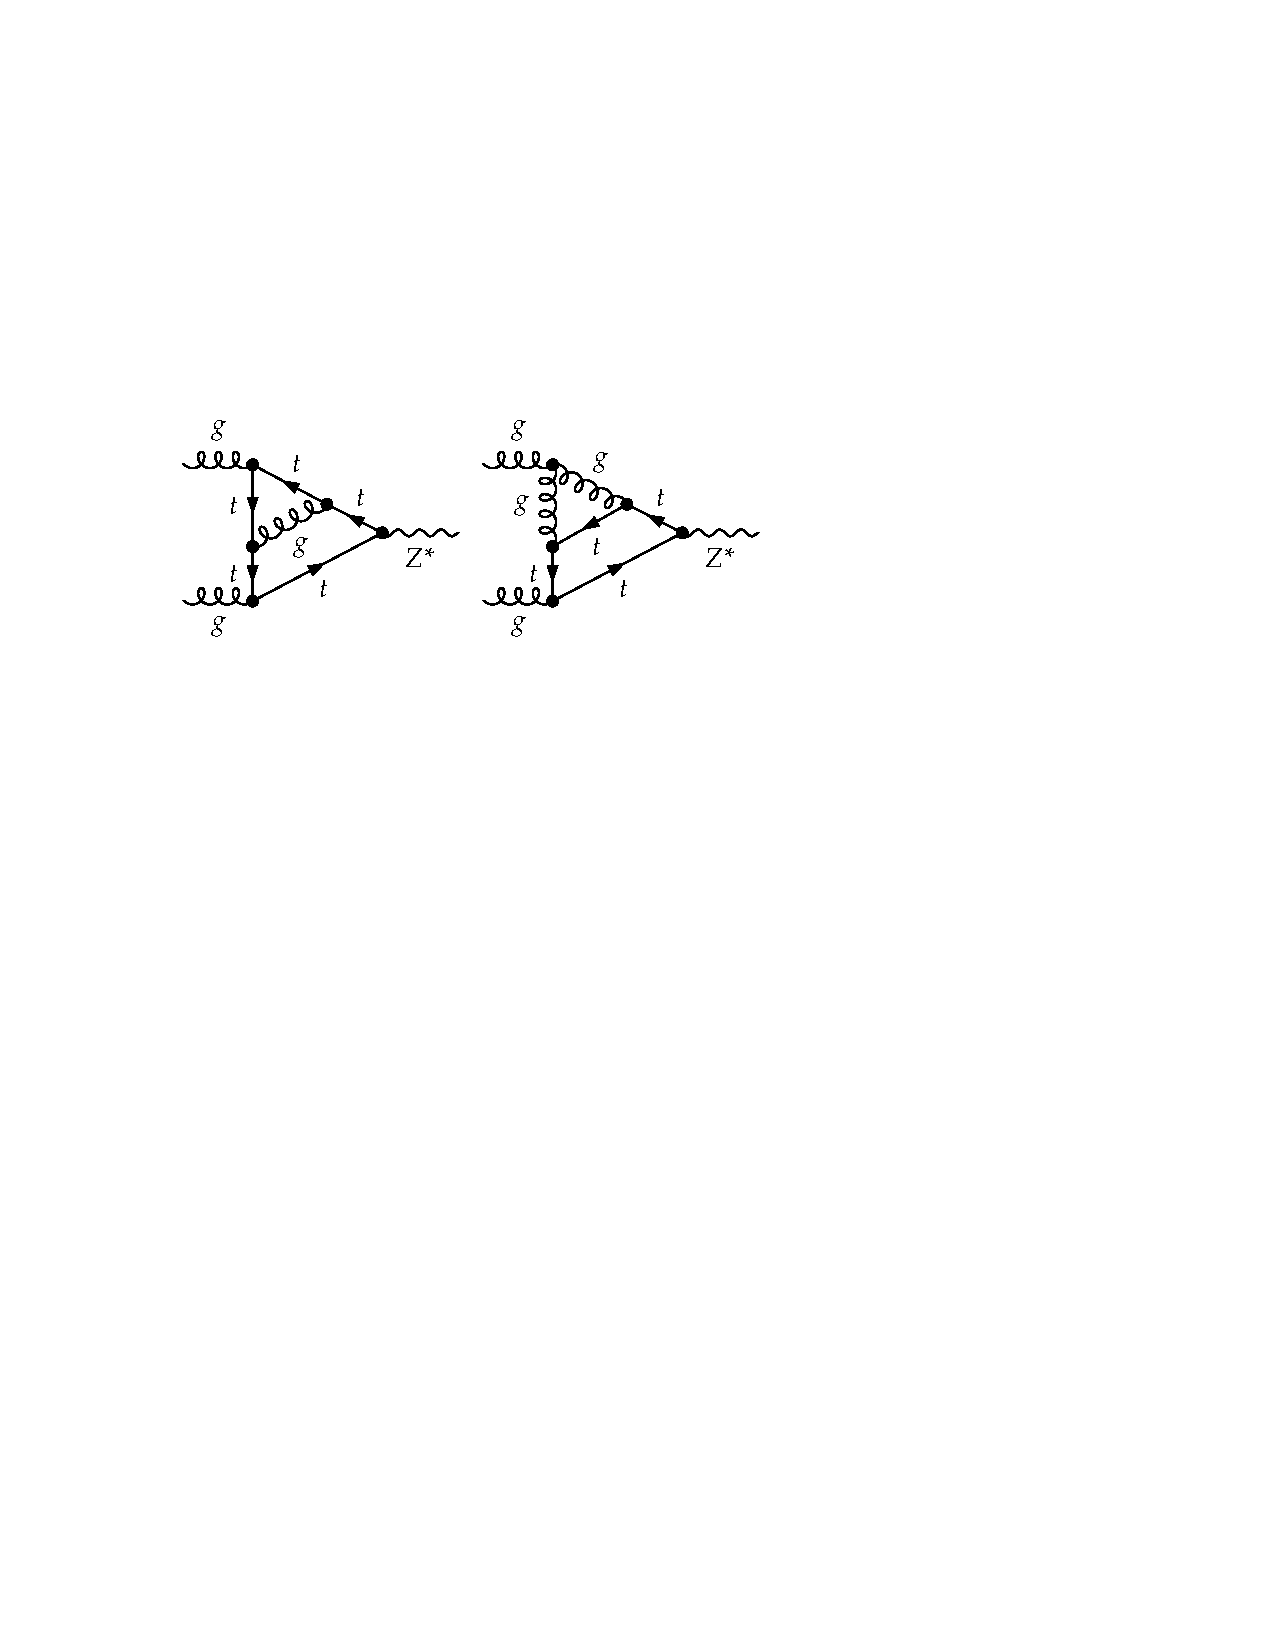
\includegraphics[width=1.2\textwidth]{2loop} 
	\end{center}
\end{minipage}
Modification on these topics may occur depending on the preliminary studies to be made prior to each project, and depending on the time.
  \section*{Goals}
   \begin{itemize}
  	\item Improve the understanding the relation between Higgs physics, EW and flavour physics.
  	\item Expand the interest in the search for Higgs pair production at the HL-LHC, by motivating its importance in probing light flavour -Higgs couplings and its non-linearity.
  	\item Explore more models and more channels for light flavour and Higgs coupling, e.g $ h WW$ and $h ZZ$ production.
    \item Provide an analytical calculation for the quantum correction in QCD  at order $\alpha_s^4$for the process $ gg \to hZ$ and explore the potential application of the computed amplitudes for exploring NP scenarios with heavy leptonic states.
  \end{itemize}
 \section*{Literature review}
 \subsection*{Higgs pair production via gluon fusion}
\par The dominant process for Higgs pair production at the LHC~(and hadron colliders in general) is the gluon gluon fusion~(ggF) via a heavy quark loop~$Q$, mainly the top and beauty quark, with the latter contributing only to about~$1\%$, see figure~\ref{fig_ggf_sm}.
 %
 \begin{figure}[!htpb]
 	\centering
 	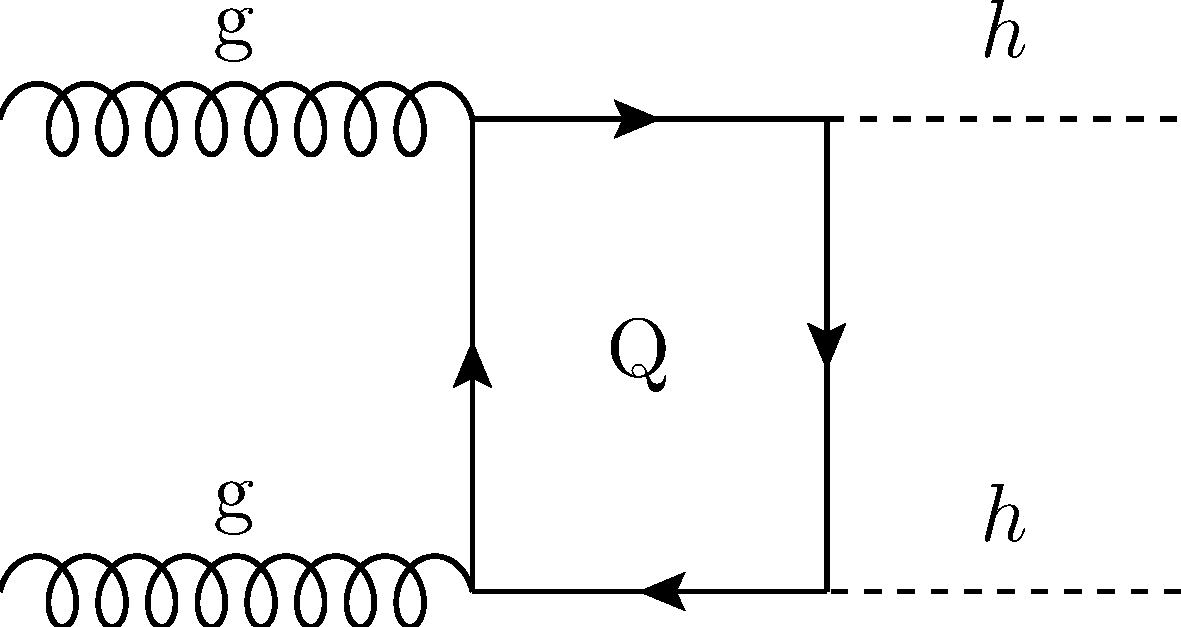
\includegraphics[width = 0.25\textwidth]{ggfbox}
 	\hspace{0.3 cm}
 	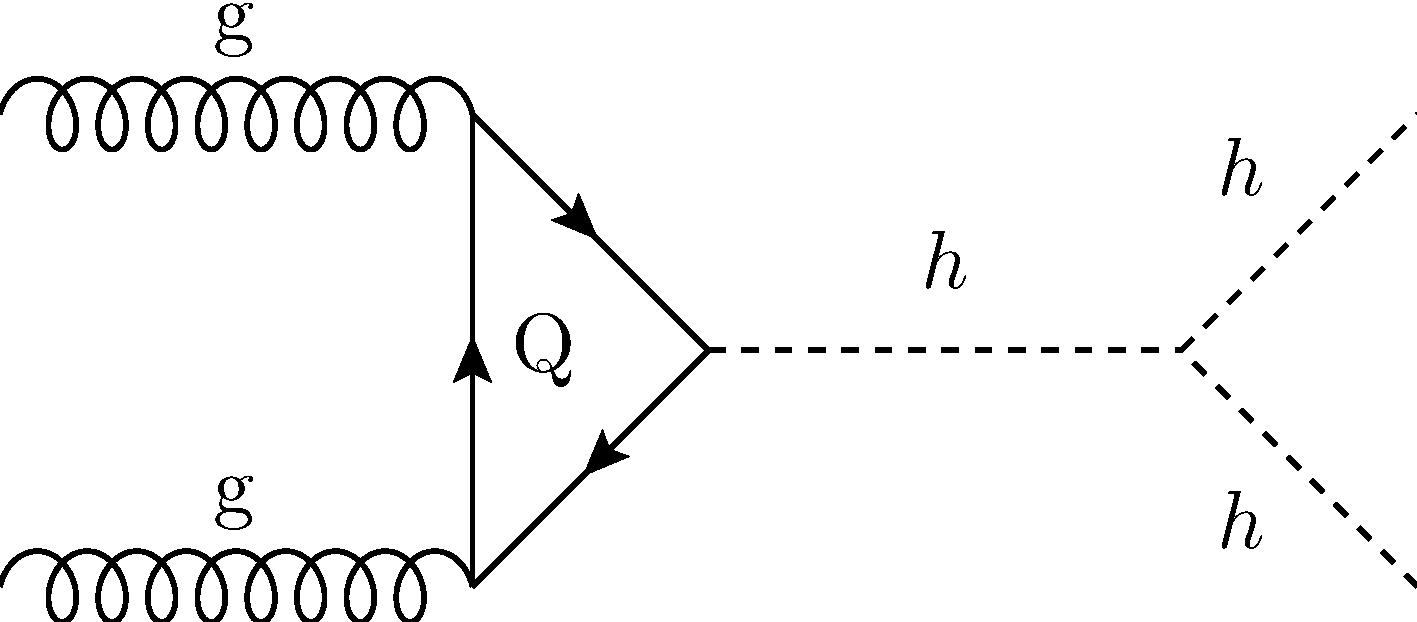
\includegraphics[width = 0.3\textwidth]{ggftri}
 	\caption{Feynman diagrams for the ggF process of Higgs pair production in the SM.} % verify the notation
 	\label{fig_ggf_sm}
 \end{figure}
 %
  This process is well-studied at leading order~(LO) analytically \cite{EBOLI1987269,GLOVER1988282,DICUS1988457,Plehn:1996wb}. The next-to-leading  QCD order~(NLO)   was initially computed using infinite top mass limit~($m_t \to \infty$) using the Higgs effective field theory~(HEFT) and implemented in the programme \texttt{Hpair}~\cite{Dawson:1998py}. However, this approximation is not suitable for obtaining distributions, and using numerical methods~\cite{Borowka:2016ypz,Borowka:2016ehy,Baglio:2018lrj} the full NLO results were obtained. In ~\cite{Heinrich:2019bkc}, parton shower effects were included in the NLO calculations, allowing the use of the NLO in event generators such as \textsc{Pythia} and \textsc{Powheg}. Analytical calculations for the NLO corrections using small Higgs transverse momentum~$p_{T,h} \to 0$ yielded a good estimation for the numerical result~\cite{Bonciani:2018omm}. The use of Pad\'e approximation obtained also analytical results for the NLO result and a description for the three-loop~(NNLO) form factors~\cite{Davies:2019nhm}. The NNLO cross section with top mass effects has been computed numerically in~\cite{Grazzini:2018bsd}.
 %
\subsection*{Searches for modified light fermion couplings to the Higgs} 
\par  Yukawa interaction between the Higgs and quark and leptons does not originate from fundamental principles of the SM, and poses a puzzle to explain their origin and hierarchy. Many New Physics~(NP) models predict modified /enhanced Yukawa couplings such as models with general minimal flavour violation~\cite{PhysRevD.80.076002}, vector-like fermions that cause Higgs mediated flavour violation~\cite{Giudice:2008uua,Bar-Shalom:2018rjs}, supersymmetry~\cite{Dery:2014kxa}, little Higgs models~\cite{Dib:2005re}, composite Higgs models~\cite{Carmona:2013cq,Gillioz:2013pba,Delaunay:2013iia,Delaunay:2013pwa}, 2HDM with spontaneous flavour violation~\cite{Egana-Ugrinovic:2018znw, Egana-Ugrinovic:2019dqu}, 2HDM with generic Yukawa coupling c.f.~\cite{Crivellin:2013wna}  or even with RS gravitons~\cite{vonHarling:2016vhf}, see figure~\ref{fig_uv_qqhh}
\begin{figure}[!h]
	\centering
	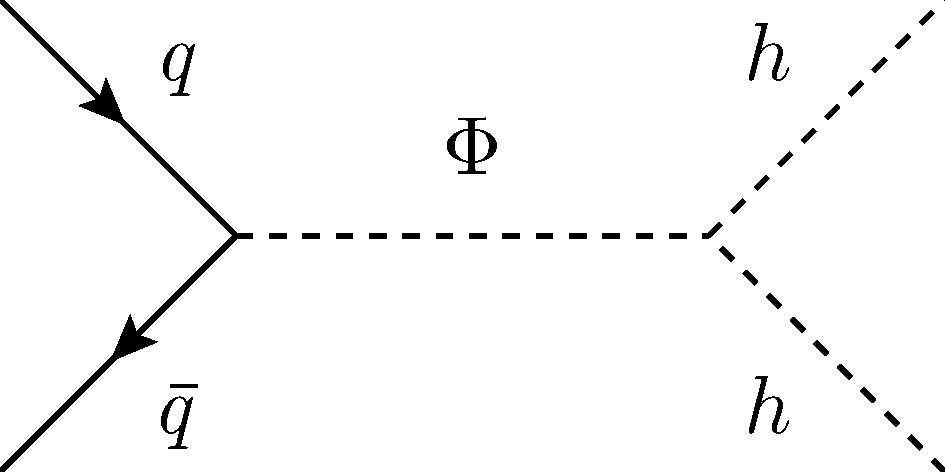
\includegraphics[width = 0.25\textwidth]{qqh_2hdm_prpg}
	\hspace{0.5 cm}
	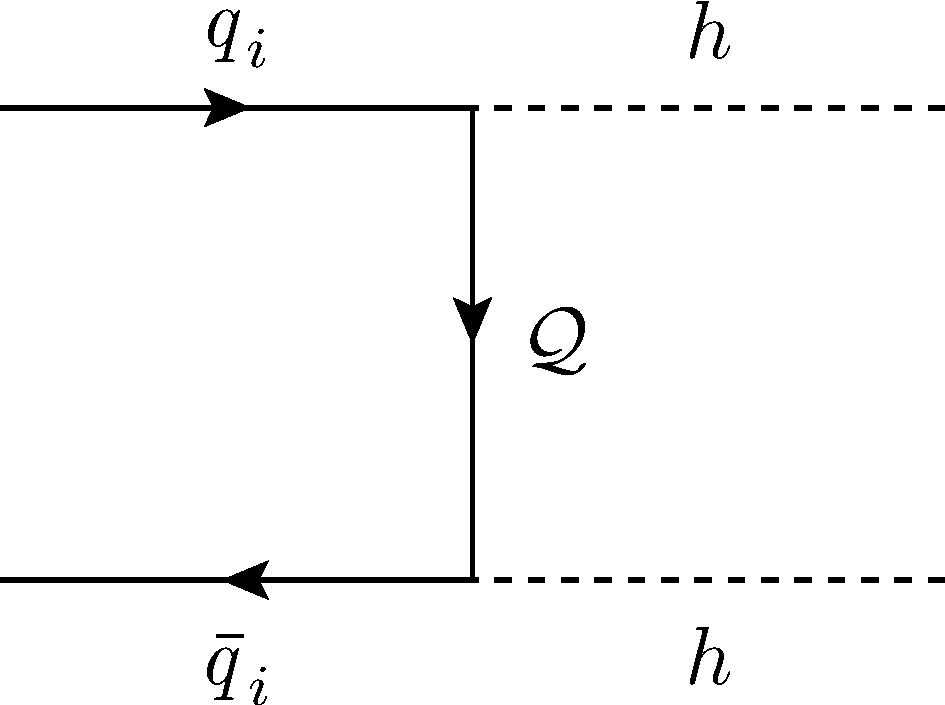
\includegraphics[width = 0.2\textwidth]{VLQ}
	\caption{Examples of potential UV-complete models leading to a  $hh f \bar{f} $ coupling. The left Feynman diagram shows a heavy Higgs $H$, the right diagram a vector-like quark $\mathcal Q $.} % verify the notation
	\label{fig_uv_qqhh}
\end{figure}
Unlike the case for the trilinear coupling, perturbative unitarity offers a very weak bounds for the fermion mass generation scale for light flavours of $ \Lambda \sim \sqrt{v^3/m_f}\sim 20$TeV~\cite{PhysRevLett.59.2405,Dicus:2004rg}, which do not constrain the above mentioned models in any significant way. \\
\par Direct searches for the decay $ h\to \bar c c$ has been made by CMS~\cite{CMS-PAS-HIG-18-031}, and ATLAS~\cite{ATL-PHYS-PUB-2018-016}, resulting in a bound on the charm Yukawa coupling $\kappa_c < 37$ at 95\% CL. Mesurment of the decay $h\to \tau^- \tau^+$ has been made by both ATLAS and CMS~\cite{Sirunyan:2017khh,Aaboud:2018pen}. While searches for the mode $ h\to \mu^- \mu^+$  resulted in an upper limit on $\kappa_\mu < 2.92$ at 95\% CL~\cite{Sirunyan:2018hbu,ATLAS-CONF-2019-028}.\\
\par  Indirect experimental constrains on the Yukawa couplings of the light quarks~(i.e. first and second generations) were constrained from current Higgs data~ \cite{Kagan:2014ila, Perez:2015aoa}, and prospects for the HL-LHC~\cite{deBlas:2019rxi}, based on a model-dependent global fit. Where the expected HL-LHC 95\% CL sensitivity bounds are 
  \begin{equation*}
 |\kappa_u|< 570\,, \hspace*{0.5cm} |\kappa_d|< 270\,, \hspace*{0.5cm}|\kappa_s|< 13\,, \hspace*{0.5cm} |\kappa_c |< 1.2\, , 
 \end{equation*}
where  $\kappa_q$ being the ratio between the expected measured couplings and the SM prediction, for a given quark flavour $q$.\\   In addition for these bound being rather ``loose", the made with certain ansatz on the Higgs width~ \cite{Caola:2013yja}  or the energy dependence of these couplings~\cite{Englert:2014aca}. These fits are only concerning the $\kappa$-formalism originating form the SMEFT and assuming linear relation between the  $h \bar f f$ (Yukawa) and  $h h \bar f f$ , and does not cover the alternative model-independent chiral Lagrangian effective field theory described by~\cite{Coleman:1969sm, Callan:1969sn}, that could contain non-linear Higgs fermion interactions.
\par Another way to improve the bounds for light Yukawa is via the search of rare Higgs decays as proposed by~\cite{Bodwin:2013gca}, for example $h \to J\slash \psi \, \gamma$ with branching fraction bound $ \mathcal B$ of $0.19\%$ bound at 95\% CL~\cite{Sirunyan:2018fmm}, while the SM prediction has been computed is $ \sim 2.5 \cot 10^{-6}$, other similar decay are also possible like $h \to (\rho, \omega, \phi) \gamma$. They have also been proposed to probe non diagonal flavour coupling~(beyond minimal flavour violation)~\cite{Kagan:2014ila}. The main advantages of these process are the SM prediction for them is very small, making them rather sensitive for the modification of the Yukawa coupling. In addition to the avoidance of the need for flavour tagging, which is  particularly challenging from light flavours. 
Moreover, the rare decay have a relatively small background e.g.$Z\to M \gamma $, high selection efficiency~$ \sim 20-30\%$ and a good mass resolution $ \sim 1.2 - 1.8 \%$\cite{Aad:2015sda}.   
\par
Constraining the light quark Yukawa couplings can also be done  from studying Higgs kinematics.  If the Higgs boson is produced with an associated jet, the transverse momentum distribution changes with respect to the SM one in the presence of enhanced quark Yukawa couplings of the second and first generation. For the second generation quarks, the main effect stems from log-enhanced contributions due to interference between top and light quark loop diagrams. This allows to set a bound on $\kappa_c \in [-0.6, 3.0]$  at 95\% C.L. at the HL-LHC \cite{Bishara:2016jga}. Instead in the presence of significantly enhanced first generation quark Yukawa couplings the Higgs boson can be directly produced from initial state quarks, which again would alter the Higgs $p_{T}$-distribution \cite{Soreq:2016rae}. For non-collider probes of the light Yukawa couplings see ref.~\cite{Delaunay:2016brc}.
\subsection*{ Quantum corrections to $ pp \to Vh$ process. }
\par The dominant process for the production of $h$ associated with $Z$or $W$ bosons is via quark anti quark annihilation via a Drell-Yan~(DY) like process, with Higgsstrahlung of the off shell $Z/W$, this process was first investigated by Glashow:1978ab et al.~\cite{Glashow:1978ab} and the first QCD corrections by~\cite{Han:1991ia}. This is at a tree-level, hence the leading order cross-section is at $\alpha_s$ order. NNLO QCD corrections to this process's cross-section $\mathcal O(\alpha_s^4)$  has been computed by~\cite{vanNeerven:1991gh,Brein:2003wg,Brein:2004ue}, and found to be a $ 1-3\%$ correction . Later on, the full differential distribution was studied for example in~\cite{Ferrera:2014lca}. 
\par The gluon fusion process $gg \to Vh$ is considered an NLO correction at one loop as its cross section contribution  is of order $\mathcal O(\alpha_s^2)$, it has first been calculated by~\cite{Dicus:1988yh,Kniehl:1990iva,Brein:2003wg,Brein:2004ue} which has a $5\%$ correction. The 2 loop QCD correction has been computed in the infinite top mass limit by ~\cite{Altenkamp:2012sx}, they have found that the K-factor to the 1 loop process is $\sim 2$ which makes this NNLO correction comparable to the NNLO correction to the DY-like process, with significant renormalisation scale dependence. In the  infinite top mass limit however, it is unreliable for studying distributions as this approximation becomes invalid when $ s =M_{Zh}^2 > 4m_t^2$.  Top quark- mediated corrections of order $ \sim g_2^3 \lambda_t \alpha_s^2$ has been recently calculated to be $\sim 1-2\%$~\cite{Brein:2011vx}. Ciccolini et al. and Denner et al. ~\cite{Ciccolini:2003jy,Denner:2011id,}. have calculated the radiative EW corrections (NLO) has a $\sim 5\%$ contribution to the cross-section. All of these correction has been included in the programme \texttt{ vh@nnlo} ~\cite{Brein:2012ne}.

\par The  $Vh$ process has an important r\^ole in the precision measurements of Higgs couplings. Moreover, the gluon fusion $Vh$ production could be the dominant process for the production of heavy leptonic states predicted by  some NP models c.f.~\cite{Ruiz:2017yyf}.
%\subsection*{ Constraining $\lambda_{hhh}$ from single Higgs production }
% bla bla
 \section*{Work plan and milestones }
 \subsection*{First year: March 2019- March 2020}
Milestones;
 \begin{itemize}
 \item The project : Probing Higgs couplings to light quarks via Higgs pair production, has been completed. \\
 A paper was published : see~\cite{Alasfar:2019pmn}, along with a proceeding~\cite{Alasfar:2019wby}. Contribution with this project in few conferences and workshops : EPS-HEP 2019, LHC-HH working group meeting and Berlin COAST workshop.
 \item The project : Next-to-leading order~(NLO) QCD correction to $Zh$ production via gluon fusion  with full top mass effect\\ Virtual (2loop) corrections to the triangle diagram has been completed. 
 \item The project:  One-loop New Physics scenarios for $b \to s$ anomalies: Combining EW and Flavour constraints in the SMEFT \\ Almost completed, remaining only the completion of the paper preprint. 
 \end{itemize}
 \subsection*{Second year: April 2020- March 2021}
Upcoming;
 \begin{itemize}
 	\item The project : Next-to-leading order~(NLO) QCD correction to $Zh$ production via gluon fusion  with full top mass effect\\ Real corrections to the triangle are being computed, will be done by 15.05.2020.  
 	\item The project:  One-loop New Physics scenarios for $b \to s$ anomalies: Combining EW and Flavour constraints in the SMEFT \\  Completion of the paper draft and final cross-checks. Should be done by 30.05.2020. 
	\item Invited for PANIC conference in Lisbon, Aug.-Sept. 2020, to present the work done on probing Higgs couplings to light quarks via Higgs pair production.
\end{itemize}
Planned;
 \begin{itemize}
	\item Starting the project~(literature review mainly)  Investigation of the process $  pp \to h W^+ W^-$  with modified  light Yukawa coupling . Expected by June 2020. Calculations starting on  July. finish before the end of 2020. 
	\item Writing the report on the NLO corrections to  $Zh$ production via gluon fusion the triangle diagram (June-July).
	\item Depending on the results, it is possible to work on BSM physics from $gg\to Z^*$ at NLO as a separate project, to end by Sept.- Oct.
	\item Waiting for the box diagrams of $Zh$ to be completed. in order to complete (to be determined).
\end{itemize}
 \subsection*{Third year:April 2021- March 2022}
Planned;
\begin{itemize}
	\item Work on the remaining projects, hard to specify the details early on. 
	\item There will be 3-4 months for writing the doctoral thesis and preparing for the defence. 
\end{itemize}
Remarks:
\begin{itemize}
	\item  Continuous literature review during the doctoral work time. Not just for the direct relearnt topics of the thesis but also in High-energy physics, and close topics, in general.
	\item The aim regarding conferences; is to have more or at least  keep a similar conference contribution to the first year (quality of the conference is above the quantity).
	\item In addition for the research projects, there is a teaching load of  2 teaching hours weekly (on average).
\end{itemize}

\bibliographystyle{utphys.bst}
\bibliography{bibliography}

\end{document}
